\scanpage{96}
\diagram{\begin{tikzcd}[ampersand replacement=\&,column sep=small,row sep=tiny]
\overset{\circ}{P}{}^{\unsure{\#|+}}\&\subset\&P^\#\&\subset\&\overline{P^\#}\\
\cup\&\&\&\&\cup\\
\overset{\circ}{Q}{}^\#\&\subset\&Q^+\&=\&\overline{Q^\#}\\
\cup\&\&\&\&\cup\\
\overset{\circ}{\overline R}\&=\&R\&\subset\&\overline R
\end{tikzcd}}

\[
 \boxed{\overset{\circ}{Q}{}^\#\subset P^\#}\qquad\text{d'où}\quad Q^\#=\overline{Q^\#}\subset\overline{P^\#}
\]
\margin{\uline{Prop} de \uline{\unsure{Groth|Groth.}}}
\[
 (\text{donc}\quad \overset{\circ}{Q}{}^\#\subset\overset{\circ}{\overline{P^\#}}=\overset{\circ}{P}{}^\#)
\]
d'où par polarité, comme $Q^+=Q^{+\circ}$
\[
 \overline{P^\#}{}^\circ=P^{\#\circ}\subset Q^\#
\]

\[
 P^+\ni x\Longleftrightarrow \exists\ C>0,\ \inserted{n>0}\ \text{tel que}\quad\gamma(C)=nx
 \Longleftrightarrow
 \boxed{\begin{gathered}\deleted{\text{\unsure{(si $x$ a lieu)}}}\\ \ell(nx)\geq2\ \text{si}\\ n\ \text{grand}\end{gathered}}
\]
\[
 Q^+\ni x\Longleftrightarrow
 \left\{\begin{aligned}x^2&\geq0\\x.a&\geq0\end{aligned}\right.,
 \qquad\overset{\circ}{Q}{}^\#\ni x\Longleftrightarrow x^2>0,\ x.a\geq0
\]
[$a$ choisi dans $\deleted{\unsure{R}}Q^\#$ \unsure{,} p.ex $a$ dans $R$]
\[
 R\ni x\Longleftrightarrow\exists\ C\ \text{\uline{ample}},\ n>0,\ \text{tel que}\quad\gamma(C)=nx
\]

\[
 \boxed{x\in R\ \underset{\substack{\text{th. de}\\\text{Nakai}}}{\Longleftrightarrow}\ \deleted{\unsure{x.P}}\quad x.P>0\quad\text{et}\quad x^2>0}
\]
\figure{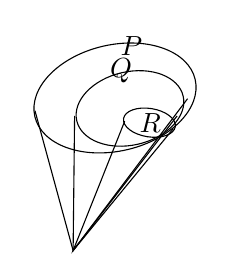
\begin{tikzpicture}[x=.95cm,y=.95cm]
\draw[rotate around={13:(0,1.7)}] (0,1.7) ellipse (1.10 and .71);
\draw[rotate around={13:(.20,1.56)}] (.20,1.56) ellipse (.73 and .49);
\draw[rotate around={-9:(.46,1.37)}] (.46,1.37) ellipse (.35 and .19);
\draw (-1.07,1.53)--(-.56,-.34)--(.97,1.69);
\draw (-.54,1.46)--(-.56,-.34)--(.83,1.46);
\draw (.13,1.39)--(-.56,-.34)--(.78,1.29);
\node at (.22,2.39) {$P$}; \node at (.08,2.07) {$Q$}; \node at (.47,1.37) {$R$};
\end{tikzpicture}}

\[
 \overline R\subset\deleted{\unsure{\bar{\phantom P}}}P^\circ\cap Q=P^\circ=\overline P{}^\circ,\quad\deleted{\unsure{a}}\quad\text{d'où}
\]
\[
 \deleted{\boxed{R\subset\unsure{P|\overset{\circ}{P}}}\quad\unsure{\text{donc}}\ P^\circ}
\]
\[
 R=\overset{\circ}{\overline R}\subset\overset{\circ}{\overline{P^\circ}},
 \qquad\text{je dis qu'on \uline{a égalité}, car}
\]
\[
 \overset{\circ}{P^\circ}\subset\overset{\circ}{Q}\quad\text{et on applique le critère de Nakai}
\]
\[
 \boxed{\begin{aligned}
 R&=\overset{\circ}{\overline{\unsure{R|K}}}=\overset{\circ}{\overline{P^\circ}}\subset\overset{\circ}{Q}\\
 \overline R&=P^\circ=\overline P{}^\circ\subset Q
 \end{aligned}}
\]

\uline{Question} \quad $xP>0\overset{?}{\Longrightarrow}x\in R$

Par Nakai, il reste à voir si $\underline{x^2>0}$ \unsure{Donc|Donné} $x^{\unsure{2}}\geq0$, il \unsure{reste} : voir $x^2\ne0$ On peut supposer que $x$ provient de $D$ div. tel que $D^2=0$. Mais alors $\chi(L(nD))=\chi(X)+n\chi(D)$ et $h^0(L(nD))\geq\chi(L(\unsure{n|m}D))$ pour $n$ grand par Mumford, on doit donc avoir $\chi(D)\unsure{<|\leq}0$

% archive sheet number: 95
